% \documentclass[12pt, oneside]{book} % Use oneside for theses, twoside for books
\documentclass[12pt]{article}
\usepackage{marvosym}

%...TikZ & PGF
\usepackage{pgfplots}
\pgfplotsset{compat=1.11}
\tikzset{>=latex}
\usetikzlibrary{calc,math}
\usepackage{tikzsymbols}
\usepgfplotslibrary{fillbetween}
\usetikzlibrary{decorations.markings} 
\usetikzlibrary{arrows.meta} %...APP2 for arrows as objects and images
\usetikzlibrary{backgrounds} %...For shading portions of graphs
\usetikzlibrary{patterns} %...Unit 5 Problems
\usetikzlibrary{shapes.geometric} %...For drawing cylinders in Unit 2
\usepackage{makecell} %...use \thead{} to enable line skip in table headers
\tikzset{
    mark position/.style args={#1(#2)}{
        postaction={
            decorate,
            decoration={
                markings,
                mark=at position #1 with \coordinate (#2);
            }
        }
    }
} %...See https://tex.stackexchange.com/questions/43960/define-node-at-relative-coordinates-of-draw-plot

\tikzset{
    declare function = {trajectoryequation10(\x,\vi,\thetai)= tan(\thetai)*\x - 10*\x^2/(2*(\vi*cos(\thetai))^2);},
    declare function = {trajectoryequation(\x,\vi,\thetai)= tan(\thetai)*\x - 9.8*\x^2/(2*(\vi*cos(\thetai))^2);},
    declare function = {patheq(\x,\yi,\vi,\thetai)= \yi + tan(\thetai)*\x - 9.8*\x^2/(2*(\vi*cos(\thetai))^2);},
    declare function = {patheqten(\x,\yi,\vi,\thetai)= \yi + tan(\thetai)*\x - 10*\x^2/(2*(\vi*cos(\thetai))^2);} %like patheq but with gravity = 10
}

%...siunitx
\usepackage{siunitx}
\DeclareSIUnit{\nothing}{\relax}
\def\mymu{\SI{}{\micro\nothing} }
\DeclareSIUnit\mmHg{mmHg}
\DeclareSIUnit{\mile}{mi}
%...NOTE: "The product symbol between the number and unit is set using the quantity-product option."

%...Other
\usepackage{amsthm}
\usepackage{amsmath}
\usepackage{amssymb}
\usepackage{cancel}
\usepackage{subcaption}
\usepackage{dashrule}
\usepackage{enumitem}
% \usepackage{fontawesome}
\usepackage{fontawesome5}
\usepackage{multicol}
\usepackage{glossaries}
%\numberwithin{equation}{section}
\numberwithin{figure}{section}
\usepackage{float}
\usepackage{twemojis} %...twitter emojis
\usepackage{utfsym}
\usepackage{linearb} %...For \BPwheel in Unit 8
\newcommand{\R}{\mathbb{R}} %...real number symbol
\usepackage{graphicx}
\usepackage{mdframed} %...For FRQ teacher boxes
\graphicspath{ {../Figures/} }
\usepackage{hyperref}
\hypersetup{colorlinks=true,
    linkcolor=blue,
    filecolor=magenta,
    urlcolor=cyan,}
\urlstyle{same}
\newcommand{\hdashline}{{\hdashrule{\textwidth}{0.5pt}{0.8mm}}}
\newcommand{\hgraydashline}{{\color{lightgray} \hdashrule{0.99\textwidth}{1pt}{0.8mm}}}

%...Miscellaneous user-defined symbols
\newcommand{\fnet}{F_{\text{net}}} %...For net force
\newcommand{\bvec}[1]{\vec{\mathbf{#1}}} %...bold vector
\newcommand{\bhat}[1]{\,\hat{\mathbf{#1}}} %...bold hat vector
\newcommand{\que}{\mathord{?}}  %...Question mark symbol in equation env
%...Define thick horizontal rule for examples:
\newcommand{\hhrule}{\hrule\hrule}
\let\oldtexttt\texttt% Store \texttt
\renewcommand{\texttt}[2][black]{\textcolor{#1}{\ttfamily #2}}% 

%...For use in the exam document class
\newif\ifprintmetasolutions


%...Decreases space above and below align and gather enironment
\makeatletter
\g@addto@macro\normalsize{%
  \setlength\abovedisplayskip{-3pt}
  \setlength\belowdisplayskip{6pt} 
}
\makeatother






\usepackage{textcomp}
\usepackage{tcolorbox}
\tcbuselibrary{raster}





% --- Packages ---
\usepackage[utf8]{inputenc}
\usepackage[T1]{fontenc}
\usepackage{lmodern} % or any other font package you like
\usepackage{geometry}
\usepackage{setspace}
\usepackage{hyperref}
\usepackage{graphicx}
\usepackage{amsmath, amssymb}
\usepackage{epigraph}
\usepackage{enumitem}
\setlength{\epigraphwidth}{0.5\textwidth}


% --- Page Geometry ---
\geometry{margin=1in}
\doublespacing %\onehalfspacing % or \doublespacing if required by guidelines

% --- Metadata ---
% \title{High School Physics Curriculum in LaTeX}
% \author{Luis Nunez}
% \date{Month Year} % e.g., May 2025

\usepackage{listings}
\usepackage{xcolor}

\definecolor{codegreen}{rgb}{0,0.6,0}
\definecolor{codegray}{rgb}{0.5,0.5,0.5}
\definecolor{codepurple}{rgb}{0.58,0,0.82}
\definecolor{backcolour}{rgb}{0.95,0.95,0.92}

\lstdefinestyle{mystyle}{
    backgroundcolor=\color{backcolour},   
    % commentstyle=\color{codegreen},
    % emph=[1]{\begin,\end},
    % emphstyle=[1]\color{blue},
    % emph=[2]{\vec,\},
    % emphstyle=[2]\color{magenta},
    % keywordstyle=\color{magenta},
    % numberstyle=\tiny\color{codegray},
    % stringstyle=\color{codepurple},
    basicstyle=\ttfamily\footnotesize,
    % breakatwhitespace=false,         
    % breaklines=true,                 
    % captionpos=b,                    
    % keepspaces=true,                 
    numbers=left,                    
    % numbersep=5pt,                  
    % showspaces=false,                
    % showstringspaces=false,
    % showtabs=false,                  
    % tabsize=2
}

\lstset{style=mystyle}

% --- Begin Document ---
\begin{document}

% \maketitle

% --------- COVER PAGE (custom) ---------
\begin{titlepage}
    \begin{center}
        \vspace*{1cm}
        {\Huge\bfseries A Common Curriculum\\for High School Physics at CFISD\par}
        \vspace{1cm}
        {\Large \bfseries by Luis Ernesto Nu\~{n}ez\par}
    \end{center}
    \vspace{1cm}
    {\large A Project Submitted in Partial Fulfillment of the Degree of\\Master of Science Teaching\\
    Department of Physics and Astronomy\\
    Rice University}
    
    \vspace{1cm}
    
    {\large \noindent Date:
    
    \vspace{1cm}
    
    \noindent Advisor: Prof.\,Patricia Reiff, Physics \& Astronomy
    
    \vspace{1cm}
    \noindent Committee Members:
    }
\end{titlepage}

% --------- FRONT MATTER ---------
% \frontmatter

% --- Abstract ---
\section*{Abstract}
This is where you write your abstract. It should summarize the project goals, methods, results, and significance.

% --- Acknowledgments ---
\section*{Acknowledgments}
Thank those who contributed to your project: advisor, family, colleagues, institutions, etc.

% --------- TABLE OF CONTENTS ---------
\tableofcontents
\clearpage

% --------- MAIN MATTER ---------
% \mainmatter

% --- Body of Project ---
\epigraph{A ``file'' was originally---in sixteenth-century England---a wire on which slips and bills and notes and letters could be strung for preservation and reference. Then came file folders, file drawers, and file cabinets; then the electronic namesakes of all these; and the inevitable irony. Once a piece of information is \textit{filed}, it is statistically unlikely ever to be seen again by human eyes.}{James Gleick, \emph{The Information}}

\epigraph{Technologies are not mere exterior aids but also interior transformations of consciousness, and never more than when they affect the word.}{Walter Ong, \emph{Orality and Literacy}}

\section{Purpose and Background}
In 1906, \textit{A First Course in Physics}, one of the first modern physics textbooks, was published by Robert A. Millikan, the physicist who a few years later would partner with Harvey Fletcher to experimentally determine the charge on an electron. In the preface, he writes that the textbook ``has grown out of the actual needs of the elementary work in physics in the University of Chicago, particularly in the University High School of the School of Education and the affiliated secondary schools.'' Millikan writes that the book represents an aim ``to make high-school physics \ldots \textit{a simple and immediate presentation, in language which the student already understands, of the hows and whys of the physical world in which he lives}.'' Three chapters of this text cover much of the first semester of a modern high school physics course:

\begin{itemize}[topsep=-2pt,itemsep=-2pt]
    \item \texttt{CHAPTER I. MEASUREMENT.} (11 pages)
    \begin{itemize}[topsep=-2pt,itemsep=-2pt]
        \item[] Fundamental Units
        \item[] Construction of Standards
        \item[] Density
    \end{itemize}
    
    \item \texttt{CHAPTER II. FORCE AND MOTION.} (26 pages)
    \begin{itemize}[topsep=-2pt,itemsep=-2pt]
        \item[] Definition and Measurement of Force
        \item[] Composition and Resolution of Force
        \item[] Gravitation
        \item[] Uniformly Accelerated Motion
        \item[] Newton's Laws
    \end{itemize}

    \item \texttt{CHAPTER VIII. WORK AND MECHANICAL ENERGY.} (21 pages)
    \begin{itemize}[topsep=-2pt,itemsep=-2pt]
        \item[] Definition of Work
        \item[] Work and the Pulley
        \item[] Work and the Lever
        \item[] The Principle of Work
        \item[] Power and Energy
    \end{itemize}
\end{itemize}

%...Link: https://books.google.com/books?id=PLYXAAAAIAAJ&printsec=frontcover&source=gbs_ge_summary_r&cad=0#v=onepage&q=momentum&f=true


% \begin{quote}
%     primarily an attempt to give concrete expression to a rapidly spreading movement to make high-school physics, to a less extent that it has been in the past, either a condensed reproduction of college physics, or a mathematical and mechanical introduction to technical science, and to a greater extent than it has heretofore been, \textit{a simple and immediate presentation, in language which the student already understands, of the hows and whys of the physical world in which he lives}.
% \end{quote}

Compare this outline with the contents shown below of the widely used undergraduate textbooks of Halliday \& Resnick's \textit{Fundamentals of Physics} and Sears \& Zemansky's \textit{University Physics}, and we begin to see a common thread:

\begin{center}
\fbox{
\begin{minipage}{7cm}
    \footnotesize
    \hfill \texttt{Halliday 
    \& Resnick} \hfill \phantom{.}

    \textbf{1} Measurement\\
    \textbf{2} Motion Along a Straight Line\\
    \textbf{3} Vectors\\
    \textbf{4} Motion in Two and Three Dimensions\\
    \textbf{5} Force and Motion I\\
    \textbf{6} Force and Motion II\\
    \textbf{7} Kinetic Energy and Work\\
    \textbf{13} Gravitation
\end{minipage}
}
\hspace{2mm}
\fbox{
\begin{minipage}{8cm}
    \footnotesize
    \hfill \texttt{Sears 
    \& Zemansky} \hfill \phantom{.}

    \textbf{1} Units, Physical Quantities, and Vectors\\
    \textbf{2} Motion Along a Straight Line\\
    \textbf{3} Motion in Two or Three Dimensions\\
    \textbf{4} Newton’s Laws of Motion\\
    \textbf{5} Applying Newton’s Laws\\
    \textbf{6} Work and Kinetic Energy\\
    \textbf{7} Potential Energy and Energy Conservation\\
    \textbf{8} Momentum, Impulse, and Collisions\\
    \hspace{-2ex} \textbf{13} Gravitation
\end{minipage}
}
\end{center}

College Board follows a similar content sequence for the eight units that comprise its first-year, algebra-based advance placement course:

\begin{center}
\fbox{
\begin{minipage}{7cm}
    \footnotesize
    \hfill AP\textsuperscript{\textregistered} Physics 1 \hfill \phantom{.}

    \textbf{1} Kinematics\\
    \textbf{2} Force and Translational Dynamics\\
    \textbf{3} Work, Energy, and Power\\
    \textbf{4} Linear Momentum\\
    \textbf{5} Torque and Rotational Dynamics\\
    \textbf{6} Energy and Momentum of Rotating Systems\\
    \textbf{7} Oscillations\\
    \textbf{8} Fluids
\end{minipage}
}
\end{center}

The underlying flow to the sequence in many of the widely used physics curricula at both the high school and college levels appears to be: kinematics first, followed by forces, energy, and momentum. Throughout the 20th century, countless secondary textbooks and resources---like the \texttt{PhysicsClassroom.com}, Khan Academy, and \texttt{FlippingPhysics.com}---adopted the sequence outlined above as the underlying logic of their curricula. Moreover, tens of thousands of physics teachers and physics majors were academically nurtured to internalize the kinematics-forces-energy-momentum schema; myself included. As a freshman undergraduate physics major at the California State University Los Angeles, I found my first exposure to college-level mechanics in Sears \& Zemanzsky's \textit{University Physics}. Later, when I transferred to Cal Poly Pomona, I learned a ton of modern physics from Halliday and Resnick's \textit{Fundamentals of Physics}, a text which I still frequently reference to this day when teaching high school physics. Thousands of teachers or former students today know, or once knew, the outline of this ``traditional'' sequence of physics contents.

But beginning in 2022, curriculum coaches and administrators at the Cypress-Fairbanks Independent School District (CFISD), where I teach, began to implement a scope and sequence for their physics courses that pedagogically and structurally deviated from a traditional sequence. These educators decided it was better for high school students to learn physics through an energy-and-momentum-first approach, so that energy and momentum topics could be ``spiraled'' throughout all topics in the curriculum. The 2025-2026 scope and sequence covering about a semester and a half is outlined below:

\begin{center}
\fbox{
\begin{minipage}{7cm}
    \footnotesize
    \hfill Physics at CFISD \hfill \phantom{.}

    \textbf{1} Constant Motion\\
    \textbf{2} Force Interactions\\
    \textbf{3} Changing Motion: Law of Acceleration\\
    \textbf{4} Changing Motion: Impulse and Work\\
    \textbf{5} Force Analysis\\
    \textbf{6} 1D Motion\\
    \textbf{7} 2D Motion\\
    \textbf{8} Conservation of Mechanical Systems
\end{minipage}
}
\end{center}

The following outline fleshes out what is covered in these units and exposes why the newly proposed curriculum is a significant departure from the traditional; the list is comprehensive but not exhaustive:

\begin{itemize}[itemsep=-2pt,topsep=-2pt]
    \item Unit 1: Constant Motion
    \begin{itemize}[itemsep=-2pt,topsep=-2pt]
        \item covers kinematics of systems moving with constant or zero velocity ($a = 0$)
        \item introduces position and velocity graphs
        \item introduces kinetic energy ($K = \frac{1}{2} m v^2$)
        \item introduces momentum ($p = mv$)
        \item \textbf{\underline{DOES NOT include}} potential energy
    \end{itemize}
    \item Unit 2: Force Interactions
    \begin{itemize}[itemsep=-2pt,topsep=-2pt]
        \item introduction to forces and force pairs
        \item free-body diagrams
        \item Newton's third law and first law
        \item \textbf{\underline{DOES NOT include}} Newton's second law
        \item \textbf{\underline{DOES NOT include}} Newton's law of gravitation
    \end{itemize}
    \item Unit 3: Changing Motion: Law of Acceleration
    \begin{itemize}[itemsep=-2pt,topsep=-2pt]
        \item acceleration as $a = \frac{\Delta v}{\Delta t}$
        \item Newton's second law ($F = ma$)
        \item change in momentum
        \item change in energy
    \end{itemize}
    \item Unit 4: Changing Motion: Impulse and Work
    \begin{itemize}[itemsep=-2pt,topsep=-2pt]
        \item impulse and $F \Delta t = \Delta p $
        \item work and $W = \Delta K$
        \item power
        \item \textbf{\underline{still DOES NOT include}} potential energy
    \end{itemize}
    \item Unit 5: Force Analysis
    \begin{itemize}[itemsep=-2pt,topsep=-2pt]
        \item Newton's law of universal gravitation
        \item weight and the gravitational field
        \item the normal force
        \item writing net force equations from free-body diagrams
        \item \textbf{\underline{DOES NOT introduce}} the laws of motion (see previous units).
    \end{itemize}
    \item Unit 6: 1D Motion
    \begin{itemize}[itemsep=-2pt,topsep=-2pt]
        \item momentum, energy, and kinematics of accelerated motion
    \end{itemize}
    \item Unit 7: 2D Motion
    \begin{itemize}[itemsep=-2pt,topsep=-2pt]
        \item momentum, energy, and kinematics of projection motion 
        \item momentum, energy, and kinematics of circular motion
    \end{itemize}
    \item Unit 8: Conservation of Mechanical Systems
    \begin{itemize}[itemsep=-2pt,topsep=-2pt]
        \item \textbf{\underline{first} introduction to} potential energy
        \item conservation of momentum
        \item conservation of energy
    \end{itemize}
\end{itemize}

For a physics major like me---whose schema of foundational physics knowledge flows from kinematics to forces, to energy, and to momentum---the deconstruction and re-construction of a physics curriculum as listed above may be a bit disorienting. My biggest challenge in learning to adopt the non-traditional sequence was the de-compartmentalization of forces and potential energy. The CFISD sequence covers many elementary ideas related to forces, but it scatters them across 3 or 4 units. For example, Newton's third law and first law are covered in Unit 2, but a student must wait till the next unit to learn about the second law. One must wait until Unit 5 to learn about the law of gravitation and net force equations, and it is forbidden to teach gravitational potential energy until the spring semester, where it is covered in Unit 8. Also, a teacher must remember to spiral in connections to momentum and energy, which were covered in the first unit, whenever possible in each of the subsequent units. The roadmap of the CFISD physics curriculum may appear confusing to a novice teacher.

Perhaps the biggest challenge of adopting the CFISD physics sequence is that the content of traditional textbooks and established online resources, especially PhysicsClassroom.com (for which our district pays a subscription), cannot be easily followed in a linear way. Long established resources do not disentangle Newton's laws of motion but teach them sequentially; do not place a large content gap between kinetic energy, on the one hand, and work and potential energy, on the other; do not expect students to know about momentum and kinetic energy before they learn about acceleration and Newton's second law. So, to try to implement PhysicsClassroom.com resources or the logic of Halliday \& Resnick's \textit{Fundamentals of Physics} in the CFISD curriculum is impractical. 

When this new sequence was being pitched to CFISD teachers about 5 years ago, I asked the district curriculum coach, ``It would be nice to have a general outline for how to conduct such a course. Is there some textbook that adopts this new sequence?'' She answered something to the effect of, ``There is no textbook with this sequence. This is something new we want to try. All of the resources for this sequence will need to be arranged by our teachers in our district.'' In other words, the cannon of curriculum would need to largely constructed bottom-up.

This capstone project was born out of my desire and need to create a kind of manual for physics teachers at CFISD to be able to maneuver the roadmap of the new curriculum. In conjunction with my pursuit of a Master of Science Teaching degree at Rice University, over the past two years I have been working on a curriculum project that consists of two main parts. The first part is a live and growing document of lecture notes that lays out the new CFISD sequence of physics ideas in a textbook-like format. That document partially fulfills the role of the vacant textbook, which we were told does not exist for our sequence. The second part of my capstone project consists of a large bank of carefully sequenced questions, quizzes, and tests for the new curriculum. The question bank addresses the requirement that topics must be covered in a specific order with certain ones addressed early (kinetic energy, momentum, Newton's third law) and certain others addressed later (Newton's second law, net force equations, potential energy). This bank, as opposed to those found in a standard textbook, \textit{can} and should be taught linearly, since it is design with to align with the CFISD sequence.

In sum, it's not so much the de-construction, per-se, of the traditional physics sequence by CFISD educators that is problematic; rather, it's the consequential impracticability of external resources based on a more traditional sequence that is the major issue. My capstone project seeks to provide an ounce of relief in the administration of the CFISD curriculum in my classroom, and by extension to my campus and district. 




\clearpage


\section{Methodology}
An overarching objective of this capstone project was to integrate high school physics theory, examples, diagrams, and practice problems into a unified and coherent location. \LaTeX\ was used to write all equations, draw most diagrams (\textit{TikZ} pictures), and arrange carefully selected problems to use for practice or quizzes. All \LaTeX\ code was stored and compiled in Overleaf, an online \LaTeX\ editor, and GitHub was integrated to share and frequently back-up the latest versions of the project.

\subsection*{LaTeX}

\LaTeX\ enables a teacher to neatly typeset his or her own equations and geometric diagrams. The \texttt{equation} environment was used to write equations elegantly, such as Newton's law of universal gravitation. When, in Overleaf, the block of code

\begin{lstlisting}[language=TeX]
\begin{equation}
    \vec{F}_g = -\frac{G m_1 m_2}{r^2}
\end{equation}
\end{lstlisting}

\noindent is compiled, the following equation is generated:

\begin{equation}
    \vec{F}_g = -\frac{G m_1 m_2}{r^2}
\end{equation}

Aside from the \texttt{equation} environment, \texttt{tikzpicture} was the most heavily used environment. It allows a use to create geometrically oriented pictures. For example, to generate a write triangle, the following lines were written:

\begin{lstlisting}[language=TeX]
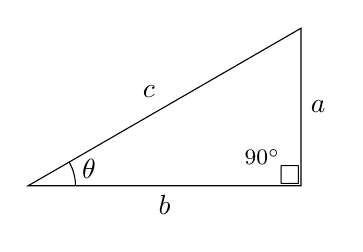
\begin{tikzpicture}[x=4cm,y=4cm]
    \draw (0,0) -- ({cos(30)},0) node[below,pos=0.5] {$b$} 
        node[above left=4pt] {\footnotesize \ang{90}} 
        -- ({cos(30)},{sin(30)}) node[right,pos=0.5] {$a$}  
        -- cycle node[above left,pos=0.5] {$c$};
    \node[shift={(-0.035,0.035)}] at ({cos(30)},0) {$\square$};
    \draw (0.15,0) arc (0:30:0.15) node[pos=0.7,right] {$\theta$};
\end{tikzpicture}
\end{lstlisting}

\begin{center}
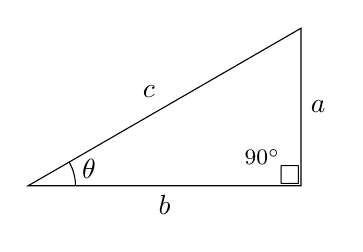
\begin{tikzpicture}[x=4cm,y=4cm]
    \draw (0,0) -- ({cos(30)},0) node[below,pos=0.5] {$b$} 
        node[above left=4pt] {\footnotesize \ang{90}} 
        -- ({cos(30)},{sin(30)}) node[right,pos=0.5] {$a$}  
        -- cycle node[above left,pos=0.5] {$c$};
    \node[shift={(-0.035,0.035)}] at ({cos(30)},0) {$\square$};
    \draw (0.15,0) arc (0:30:0.15) node[pos=0.7,right] {$\theta$};
\end{tikzpicture}
\end{center}

\noindent \textit{TikZ} was used to create numerous graphs.

\begin{lstlisting}[language=TeX]
\begin{center}
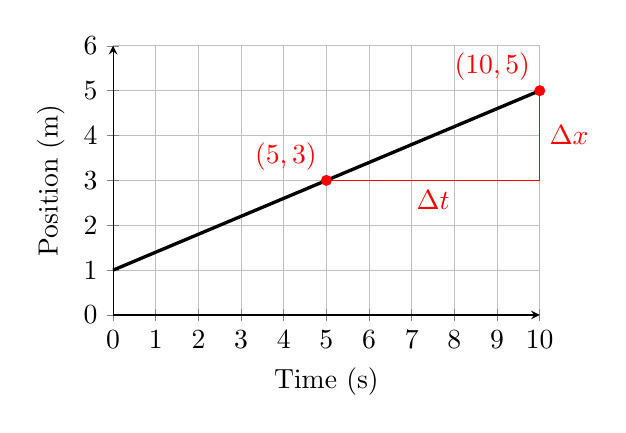
\begin{tikzpicture}
    \begin{axis}[height=5cm,width=7cm,
        axis lines=left,
        ymin=0, ymax=6,
        xmin=0, xmax=10,
        ylabel = {Position (m)},
        xlabel = {Time (s)},
        grid = both,
        ytick={0,1,...,6},
        xtick={0,1,...,10},
        clip=false
    ]
    \addplot[black,very thick,domain=0:10] {2/5*x+1}; 
    \fill[red] (5,3) circle (2pt) node[above left] {$(5,3)$};
    \fill[red] (10,5) circle (2pt) node[above left] {$(10,5)$};
    \draw[red] (5,3) -- (10,3) node[below,pos=0.5] {$\Delta t$};
    \draw[red] (10,3) -- (10,5) node[right,pos=0.5] {$\Delta x$};
\end{axis}
\end{tikzpicture}
\end{center}
\end{lstlisting}

\begin{center}
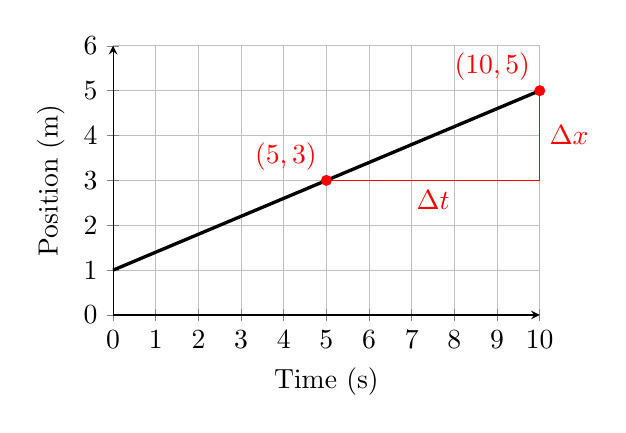
\begin{tikzpicture}
    \begin{axis}[height=5cm,width=7cm,
        axis lines=left,
        ymin=0, ymax=6,
        xmin=0, xmax=10,
        ylabel = {Position (m)},
        xlabel = {Time (s)},
        grid = both,
        ytick={0,1,...,6},
        xtick={0,1,...,10},
        clip=false
    ]
    \addplot[black,very thick,domain=0:10] {2/5*x+1}; 
    \fill[red] (5,3) circle (2pt) node[above left] {$(5,3)$};
    \fill[red] (10,5) circle (2pt) node[above left] {$(10,5)$};
    \draw[red] (5,3) -- (10,3) node[below,pos=0.5] {$\Delta t$};
    \draw[red] (10,3) -- (10,5) node[right,pos=0.5] {$\Delta x$};
\end{axis}
\end{tikzpicture}
\end{center}

\noindent Free-body diagrams:

\begin{lstlisting}[language=TeX]
\begin{tikzpicture}
    \draw (0,0) -- (4,0);
    \draw[thick] (1.5,0) rectangle ++(1,1);
    \fill (2,0.5) circle (2pt);
    \draw[->] (2,0.5) -- ++(0,+1.3) node[above] {$F_\mathrm{N}$};
    \draw[->] (2,0.5) -- ++(0,-1.3) node[below] {$F_g$};
    \draw[->] (2,0.5) -- ++(+2,0) node[right] {$F_\mathrm{A}$};
    \draw[->] (2,0.5) -- ++(-2,0) node[left] {$F_f$};
\end{tikzpicture}
\end{lstlisting}

\begin{center}
\begin{tikzpicture}
    \draw (0,0) -- (4,0);
    \draw[thick] (1.5,0) rectangle ++(1,1);
    \fill (2,0.5) circle (2pt);
    \draw[->] (2,0.5) -- ++(0,+1.3) node[above] {$F_\mathrm{N}$};
    \draw[->] (2,0.5) -- ++(0,-1.3) node[below] {$F_g$};
    \draw[->] (2,0.5) -- ++(+2,0) node[right] {$F_\mathrm{A}$};
    \draw[->] (2,0.5) -- ++(-2,0) node[left] {$F_f$};
\end{tikzpicture}
\end{center}

In the preambles of all .tex files, a function was defined to represent the trajectory equation for projectile motion,

\begin{equation*}
    y = \left(\tan \theta_0\right)x - \frac{gx^2}{2\left(v_0 \cos \theta_0\right)^2}
\end{equation*}

\noindent as

\begin{lstlisting}[language=TeX]
\tikzset{
    declare function = {
        trajectoryequation(\x,\vi,\thetai) 
        = tan(\thetai)*\x - 9.8*\x^2/(2*(\vi*cos(\thetai))^2);
        }
}
\end{lstlisting}

\noindent so that users can draw and embellish their own trajectories easily. For example, a person aiming to strike a target 15 meters away on level ground should launch a projectile at 13 meters per second at \ang{60} above the horizontal. The figure is generated by

\begin{lstlisting}[language=TeX]
\begin{tikzpicture}[x=5mm,y=5mm]
    \draw[domain=0:14.9] node[below] {launch point} 
        plot(\x,{trajectoryequation(\x,13,60)}) 
        node[below] {target};
\end{tikzpicture}
\end{lstlisting}

\begin{center}
\begin{tikzpicture}[x=5mm,y=5mm]
    \draw[domain=0:14.9] node[below] {launch point} plot(\x,{trajectoryequation(\x,13,60)}) node[below] {target};
\end{tikzpicture}
\end{center}

\noindent If the launch point is raised 10 meters above ground and the same target is to be struck, then the launch speed should be decreased to 11 meters per second:

\begin{lstlisting}[language=TeX]
\begin{tikzpicture}[x=4mm,y=4mm]
    \draw[domain=0:14.9] plot(\x,{trajectoryequation(\x,11,60) + 10}) 
        node[below] {target};
    \node[below] at (0,10) {launch point};
\end{tikzpicture}
\end{lstlisting}

\begin{center}
\begin{tikzpicture}[x=4mm,y=4mm]
    \draw[domain=0:14.9] plot(\x,{trajectoryequation(\x,11,60) + 10}) node[below] {target};
    \node[below] at (0,10) {launch point};
\end{tikzpicture}
\end{center}

\noindent Drawing circles and tangential geometry was enabled by \textit{TikZ}:

\begin{lstlisting}[language=TeX]
\begin{tikzpicture}[x=2cm,y=2cm]
    \draw[densely dashed] (0,0) circle (1);
    \draw (0,0) -- (1,0) node[below,pos=0.5] {$r$};
    \fill (0,0) circle (1pt);
    \begin{scope}[
        shift={({cos(45)},{sin(45)})},
        rotate around={45:(0,0)}]
        \draw[thick,->] (0,0) -- (0,1) node[left] {$v$};
        \draw[thick,->] (0,0) -- (-0.8,0) 
            node[above left,pos=0.8] {$a$};
        \fill (0,0) circle (3pt);
    \end{scope}
\end{tikzpicture}
\end{lstlisting}

\begin{center}
\begin{tikzpicture}[x=2cm,y=2cm]
    \draw[densely dashed] (0,0) circle (1);
    \draw (0,0) -- (1,0) node[below,pos=0.5] {$r$};
    \fill (0,0) circle (1pt);
    \begin{scope}[shift={({cos(45)},{sin(45)})},rotate around={45:(0,0)}]
        \draw[thick,->] (0,0) -- (0,1) node[left] {$v$};
        \draw[thick,->] (0,0) -- (-0.8,0) node[above left,pos=0.8] {$a$};
        \fill (0,0) circle (3pt);
    \end{scope}
\end{tikzpicture}
\end{center}

\noindent In units dealing with spring potential energy, springs were drawn:

\begin{lstlisting}[language=TeX]
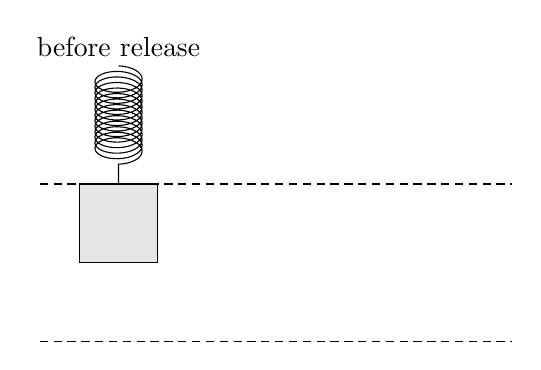
\begin{tikzpicture}
    \draw[decorate,decoration={coil,segment length=2pt,
        post length=2mm,pre length=0mm,amplitude=3mm}] 
        (0,0) node[above] {before release} -- ++(0,-1.5);
    \draw[densely dashed] (-1,-1.5) -- ++(6,0);
    \draw[densely dashed] (-1,-3.5) -- ++(6,0);
    \begin{scope}[shift={(-0.5,-2.5)}]
        \draw[fill=black!10] (0,0) rectangle (1,1);
    \end{scope}
\end{tikzpicture}
\end{lstlisting}

\begin{center}
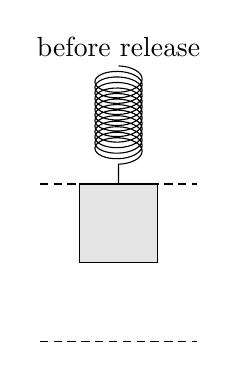
\begin{tikzpicture}
    \draw[decorate,decoration={coil,segment length=2pt,post length=2mm,pre length=0mm,amplitude=3mm}] (0,0) node[above] {before release} -- ++(0,-1.5);
    \draw[densely dashed] (-1,-1.5) -- ++(2,0);
    \draw[densely dashed] (-1,-3.5) -- ++(2,0);
    \begin{scope}[shift={(-0.5,-2.5)}]
        \draw[fill=black!10] (0,0) rectangle (1,1);
    \end{scope}
\end{tikzpicture}
\end{center}

\noindent The \verb|\usepackage{twemojis}| package allows the user to incorporate pre-generated, emoticon-type graphics to enhance visualization:

\begin{lstlisting}[language=TeX]
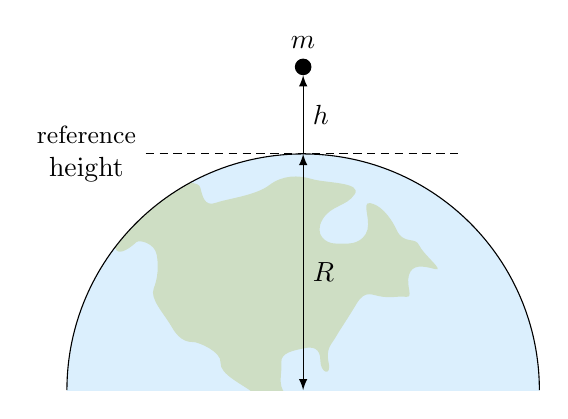
\begin{tikzpicture}
    \begin{scope}
        \clip (-3,0) -- (3,0) arc (0:180:3);
        \draw (0,0) node[opacity=0.3] 
            {\twemoji[width=6cm]{globe showing Americas}};
    \end{scope}
    \draw (3,0) arc (0:180:3);
    \draw[densely dashed] (-2,3) 
        node[left,align=center] {\small reference\\height} -- (2,3);
    \draw[<->] (0,0) -- (0,3) node[right,pos=0.5] {$R$};
    \draw[->] (0,3) -- (0,4) node[right,pos=0.5] {$h$};
    \fill[yshift=3pt] (0,4) circle (3pt) node[above=3pt] {$m$};
\end{tikzpicture}
\end{lstlisting}

\begin{center}
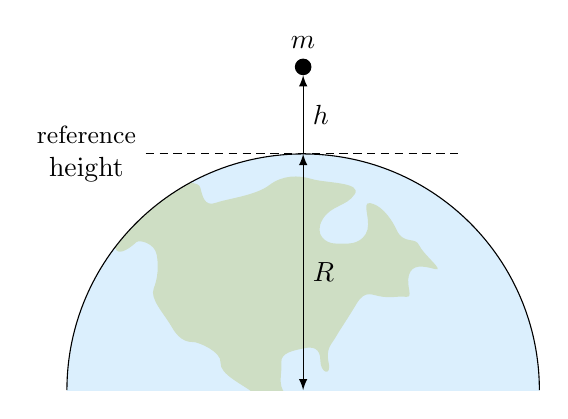
\begin{tikzpicture}
    \begin{scope}
        \clip (-3,0) -- (3,0) arc (0:180:3);
        \draw (0,0) node[opacity=0.3] {\twemoji[width=6cm]{globe showing Americas}};
    \end{scope}
    \draw (3,0) arc (0:180:3);
    \draw[densely dashed] (-2,3) node[left,align=center] {\small reference\\height} -- (2,3);
    \draw[<->] (0,0) -- (0,3) node[right,pos=0.5] {$R$};
    % \draw[<->] (0,3) -- (0,4) node[right,pos=0.5] {$y_0$};
    \draw[->] (0,3) -- (0,4) node[right,pos=0.5] {$h$};
    \fill[yshift=3pt] (0,4) circle (3pt) node[above=3pt] {$m$};
\end{tikzpicture}
\end{center}


\clearpage

\section{Results}
\subsection*{The Handbook}

\textit{The Handbook} is a 62-page (and growing) PDF document containing our high school physics sequence, definitions, foundational ideas, equations, worked examples, and graphical figures. Its creation was inspired, in part, by the work of education theorist E.D. Hirsch, who in his book \textit{The Schools We Need}, promotes the use of ``a carefully chosen but generous sampling of factual data that are set forth in a meaningful web of inferences and generalizations about the larger domain'' (Hirsch 246). \textit{The Handbook} checks all the boxes: 

\begin{itemize}
    \item its contents are chosen carefully
    \item it generously samples from up-to-date and core physics factual data
    \item it presents a ``web of inferences and generalizations'' through the coherent and logical structure of its sequence
\end{itemize}

\noindent Furthermore, it's concise and devoid of superfluous sections that are commonly found in traditional textbooks. 

Hirsch goes on to report one of the most impressive facts about education and cognitive science. He writes that ``generously selective factual instruction leads to accurate inferences not directly deducible from the literal facts that were taught'' (Hirsch 246). In other words, if there is a carefully structured system of ideas in a course, students are enabled, through pattern-recognition and induction, to make deep connections to new territories in that system. It is not necessary to cover every nook and cranny in the sphere of physics knowledge, because young minds have the capacity to extrapolate from what they already know to what they want to learn. \textit{The Handbook} provides a foundation and structure to our physics class.

The table of contents is shown below.

\fbox{\includegraphics[width=0.94\textwidth]{documents/figures/handbook-TOC-1.pdf}}

\fbox{
\includegraphics[width=0.94\textwidth]{documents/figures/handbook-TOC-2.pdf}}



% In \textit{The Schools We Need}, Hirsch recommends using ``a carefully chosen but generous sampling of factual data that are set forth in a meaningful web of inferences and generalizations about the larger domain.'' He says that ``generously selective factual instruction leads to accurate inferences not directly deducible from the literal facts that were taught.'' 
%``these selective exemplifications in order to make remarkably accurate factual guesses about untaught domains.'' (Hirsch 246).
%...Hirsch Jr, E.D.. The Schools We Need: And Why We Don't Have Them (pp. 245-246). (Function). Kindle Edition.

As mentioned in the Methodology section, \textit{The Handbook} was written entirely in \LaTeX, and, with the exception of only a few image files, all figures were generated internally from \LaTeX\ code.
\clearpage

\section{Impact}
Interpret your results and compare with literature or expectations.

\clearpage


% --- Conclusions ---
\section{Conclusions}
Summarize key insights and implications for teaching or further development.

% --------- BACK MATTER ---------
% \backmatter

% --- References ---
\section{References}
% \addcontentsline{toc}{chapter}{References and Web Links}
% \bibliographystyle{plain} % or another style: apalike, ieee, etc.
% % \bibliography{yourbibfile} % Uncomment if using BibTeX
% % Otherwise, list manually:
\begin{itemize}[topsep=0pt,itemsep=0pt]
  \item Author. *Title*. Journal, Year.
  \item \url{https://example.com}
\end{itemize}

% --- Appendix ---
% \appendix

\section{Relevant Websites}

The GitHub repository is available at \href{https://github.com/lenunez426/physics}{https://github.com/lenunez426/physics}.

\section{Appendix}
Include developed web pages, teaching activities, or supplementary material.

% \section{Additional Materials}
% Any other supporting documents or examples.

\end{document}
